\documentclass{Z}

%% packages
\usepackage{amsfonts,amstext,amsmath}
\usepackage{rotating}
%% need no \usepackage{Sweave.sty}

%% math commands
\newcommand{\R}{\mathbb{R} }
\newcommand{\Var}{\COV}
\newcommand{\V}{\COV}
\newcommand{\z}{\mathbf{z}}
\newcommand{\X}{\mathbf{X}}
\newcommand{\Y}{\mathbf{Y}}
\newcommand{\sX}{\mathcal{X}}
\newcommand{\sY}{\mathcal{Y}}
\newcommand{\T}{\mathbf{T}}
\newcommand{\x}{\mathbf{x}}
\newcommand{\y}{\mathbf{y}}
\renewcommand{\t}{\mathbf{t}}
\renewcommand{\vec}{\text{vec}}

%% code commands
\makeatletter
\newcommand\Rcmd{\bgroup\@makeother\_\@makeother\~\@makeother\$\@codez}
\def\@codez#1{{\normalfont\ttfamily\hyphenchar\font=-1 #1()}\egroup}
\makeatother
\newcommand{\Rclass}[1]{`\code{#1}'}

%% hyphenation
\hyphenation{Qua-dra-tic}

%%\VignetteIndexEntry{Implementing a Class of Permutation Tests: The coin Package}


%% JSS
\author{Torsten Hothorn \\ Ludwig-Maximilians-Universit\"at M\"unchen \And
        Kurt Hornik \\Wirtschaftsuniversit\"at Wien \AND
        Mark A.\ van de Wiel \\Vrije Universiteit Amsterdam \And
        Achim Zeileis\\Wirtschaftsuniversit\"at Wien}
\title{Implementing a Class of Permutation Tests: The \pkg{coin} Package}

\Plainauthor{Torsten Hothorn, Kurt Hornik, Mark A. van de Wiel, Achim Zeileis}
\Plaintitle{Implementing a Class of Permutation Tests: The coin Package}
\Shorttitle{Implementing a Class of Permutation Tests}

\Abstract{
  The \proglang{R} package \pkg{coin} implements a unified approach to
  permutation tests providing a huge class of independence tests  
  for nominal, ordered, numeric, and censored data as well as
  multivariate data at mixed scales. Based on a rich and flexible
  conceptual framework that embeds different permutation test procedures into a common
  theory, a computational framework is established in \pkg{coin} that
  likewise embeds the corresponding \proglang{R} functionality in a common
  \proglang{S4} class structure with associated generic functions.
  As a consequence, the computational tools in \pkg{coin} inherit
  the flexibility of the underlying theory and conditional inference
  functions for important special cases can be set up easily. 
  Conditional versions of classical tests---such 
  as tests for location and scale problems in
  two or more samples, independence in two- or three-way contingency tables,
  or association problems for censored, ordered categorical or multivariate data---
  can be easily be implemented as special cases using this computational 
  toolbox by choosing appropriate transformations of the observations.
  The paper gives a detailed exposition of both the internal structure
  of the package and the provided user interfaces.
}

\Keywords{conditional inference, exact distribution, conditional
  Monte Carlo, categorical data analysis, \proglang{R}}

\Plainkeywords{conditional inference, exact distribution, conditional
  Monte Carlo, categorical data analysis, R}




\begin{document}

\section{Introduction}

Conditioning on all admissible permutations of the data for testing 
independence hypotheses is a very old, yet very powerful and popular, 
idea \citep{fisher1935,Ernst2004}. Conditional
inference procedures, or simply \textit{permutation} or \textit{re-randomization}
tests, are implemented in 
many different statistical computing environments.
These implementations, for example 
\Rcmd{wilcox.test} for the Wilcoxon-Mann-Whitney test or
\Rcmd{mantelhaen.test} for the Cochran-Mantel-Haenszel $\chi^2$ test in the
\proglang{S} language or the tools implemented in \pkg{StatXact} \citep{StatXact6}, 
\pkg{LogXact} \citep{LogXact8}, or \proglang{Stata} \citep{Stata}
\citep[see][for an overview]{Oster2002,Oster2003},
all follow the classical classification scheme of inference procedures and
offer procedures for location problems, scale problems, correlation, 
or nominal and ordered categorical data. 
Thus, each test procedure is 
implemented separately, maybe with the exception of conditional 
versions of linear rank statistics \citep{theory-of-:-1999} in \texttt{NPAR1WAY}
as available in \proglang{SAS} \citep{SAS}.

Novel theoretical insights by \cite{StrasserWeber1999} open up the way
to a unified treatment of a huge class of permutation
tests. The \pkg{coin} package for \underline{co}nditional \underline{in}ference
is the computational counterpart to this theoretical framework,
implemented in the \proglang{R} system for statistical computing \citep{rcore2007}.
\cite{Hothorn:2006:AmStat} introduce the package and illustrate the
transition from theory to practice. Here, we focus on the design principles upon which the
\pkg{coin} implementation is based as well as on the more technical issues
that need to be addressed in the implementation of such conceptual
tools.

Formal \proglang{S4} classes describe the data model and the conditional test procedures, 
consisting of multivariate linear statistics, univariate test statistics 
and a reference distribution. Generic functions for obtaining
statistics, conditional expectation and covariance matrices as well as 
$p$~value, distribution, density and quantile functions for the reference
distribution are available. 
The most important user-visible function is  \Rcmd{independence_test},
the computational counterpart of the theoretical framework of \cite{StrasserWeber1999},
providing the same flexibility in software as in the
underlying theory. 
%%For convenience, a set of wrapper 
%%functions for the most popular test procedures, such as 2- and 
%%$K$-sample permutation tests for location or scale differences,
%%are offered as well.

\section{Theory and classes}

We first focus on the conceptual framework for conditional inference procedures
as proposed by \cite{StrasserWeber1999} along with the class structure upon which
the \pkg{coin} package is based. Formal \proglang{S4} classes defining data objects, objects describing
the inference problem and conditional test procedure are introduced and explained.

We deal with variables $\Y$ and $\X$ from sample spaces 
$\mathcal{Y}$ and $\mathcal{X}$ which may
be measured at arbitrary scales and may be multivariate as well.
In addition, $b \in \{1, \dots, k\}$, a factor measured at $k$ levels, indicates a certain block
structure of the observations: for example study centers in a
multi-center randomized clinical trial where only a re-randomization of observations within blocks
is admissible. 
We are interested in testing the null hypothesis
\begin{eqnarray*}
  H_0: D(\Y | \X, b) = D(\Y | b)
\end{eqnarray*}
of conditional independence of $\Y$ and $\X$ within blocks~$b$ against
arbitrary alternatives, for example shift or scale alternatives, linear trends,
association in contingency tables etc.

\subsection{Data} \label{sec:data}

In the following we assume that we are provided with $n$ observations 
\begin{eqnarray*}
(\Y_i, \X_i, b_i, w_i), \quad i = 1, \dots, n.
\end{eqnarray*}
In addition to variables $\X$, $\Y$, and $b$, it is convenient (for
example to efficiently represent large contingency tables)
to allow for some integer-valued case weights $w_i$, indicating
that $w_i$ observations with realizations $\Y_i$, $\X_i$ and $b_i$ 
are available, with default $w_i \equiv 1$.
This data structure is represented by class \Rclass{IndependenceProblem}:
\begin{center}
\begin{tabular}{ll}
\multicolumn{2}{l}{Class \Rclass{IndependenceProblem}} \\
 & \\
Slot & Class \\ \hline 
\code{x} & \Rclass{data.frame} \\
\code{y} & \Rclass{data.frame} \\
\code{weights} & \Rclass{numeric} \\
\code{block} & \Rclass{factor} \\
\hline
\end{tabular}
\end{center}
\subsection{Inference problem and linear statistic}

\cite{StrasserWeber1999} suggest to derive
scalar test statistics for testing $H_0$ from multivariate linear statistics
of the form 
\begin{eqnarray} \label{linstat}
\T =  \sum_{j = 1}^k \T_j \in \R^{pq}
\end{eqnarray}
where the linear statistic for each block is given by
\begin{eqnarray*}
\T_j = \vec\left(\sum_{i = 1}^n I(b_i = j) w_i g(\X_i) h(\Y_i)^\top\right)
\in \R^{pq}.
\end{eqnarray*}
The function $I(\cdot)$ is the indicator function and $\vec$
denotes the vec operator (which stacks the columns of a matrix one underneath the other).  
Here, $g: \mathcal{X} \rightarrow \R^{p \times 1}$ is a transformation of
the $\X$ measurements and $h: \mathcal{Y} \rightarrow
\R^{q \times 1}$ is called \emph{influence function}. The function $h(\Y_i)
= h(\Y_i, (\Y_1, \dots, \Y_n))$ may depend on the full vector of responses
$(\Y_1, \dots, \Y_n)$, however only 
in a permutation symmetric way, i.e., the value of the
function must not depend on the order in which $\Y_1, \dots, \Y_n$ appear.
The transformation~$g$ and influence function $h$ as well as 
$g(\X_i)$ and $h(\Y_i), i = 1, \dots, n$, are attached to the data structure
by extending class \Rclass{IndependenceProblem}:
\begin{center}
\begin{tabular}{ll}
\multicolumn{2}{l}{Class \Rclass{IndependenceTestProblem}} \\
\multicolumn{2}{l}{Contains \Rclass{IndependenceProblem}} \\
 & \\
Slot & Class \\ \hline 
\code{xtrans} & \Rclass{matrix} \\
\code{ytrans} & \Rclass{matrix} \\
\code{xtrafo} & \Rclass{function} \\
\code{ytrafo} & \Rclass{function} \\
\hline
\end{tabular}
\end{center}The \code{ytrafo} and \code{xtrafo} slots correspond to the influence
function $h$ and transformation $g$, respectively. The $i$th row of the 
$n \times q$ matrix \code{ytrans} corresponds to $h(\Y_i)$. Similar, 
the rows of \code{xtrans} ($n \times p$) correspond to $g(\X_i)$. 

In the simplest case of both $\X$ and $\Y$ being univariate 
factors at $p$ and $q$ levels, $g$ and $h$ are 
the corresponding dummy codings and the linear statistic $\T$ is the
(vectorized) $p \times q$ contingency table of $\X$ and $\Y$.

\subsection{Conditional expectation and covariance}

The distribution of $\T$  depends on the joint
distribution of $\Y$ and $\X$, which is unknown under almost all practical
circumstances. At least under the null hypothesis one can dispose of this
dependency by fixing $\X_1, \dots, \X_n$ and conditioning on all possible
permutations $S_j$ of the responses $\Y_1, \dots, \Y_n$ within block $j, j = 1, \dots, k$. 

The conditional expectation $\mu \in \R^{pq}$ and covariance 
$\Sigma \in \R^{pq \times pq}$ 
of $\T$ under $H_0$ given
all permutations $\sigma \in S$ of the responses are derived by
\cite{StrasserWeber1999} and are re-stated in the following.

Let $w_{\cdot j} = \sum_{i = 1}^n I(b_i = j)w_i$ denote the sum of the weights
in block $j$. The conditional expectation of the influence 
function $h$ in block $j$ 
\begin{eqnarray*}
\E(h | S_j) = w_{\cdot j}^{-1} \sum_i I(b_i = j)w_i h(\Y_i) \in \R^q
\end{eqnarray*}
with corresponding $q \times q$ covariance matrix
\begin{eqnarray*}
\V(h | S_j) = w_{\cdot j}^{-1} \sum_i I(b_i = j)w_i \left(h(\Y_i) - \E(h | S_j)
\right) \left(h(\Y_i) - \E(h | S_j)\right)^\top.
\end{eqnarray*}
The conditional expectation and covariance of the linear statistic
$\T_j$ in block $j$ are
\begin{eqnarray*}
\mu_j & = & \E(\T_j | S_j) = \vec \left( \left( \sum_{i = 1}^n I(b_i = j)w_i g(\X_i) \right) \E(h | S_j)^\top
\right)
\end{eqnarray*}
and
\begin{eqnarray*}
\Sigma_j & = & \V(\T_j | S_j) \nonumber \\
& = &
    \frac{w_{\cdot j}}{w_{\cdot j} - 1}  \V(h | S_j) \otimes
        \left(\sum_i I(b_i = j) w_i  \left( g(\X_i) \otimes g(\X_i)^\top\right) \right)
\label{expectcovar}
\\
& - & \frac{1}{w_{\cdot j} - 1}  \V(h | S_j)  \otimes \left(
        \sum_i I(b_i = j) w_i g(\X_i) \right)
\otimes \left( \sum_i I(b_i = j) w_i g(\X_i)\right)^\top
\nonumber
\end{eqnarray*}
respectively, where $\otimes$ is the Kronecker product. The conditional
expectation and covariance of $\T$, aggregated over all $k$ blocks, are
then given by
\begin{eqnarray*}
\E(\T | S_j) & = & \mu  \; = \; \sum_{j = 1}^k \mu_j  \; = \; \sum_{j = 1}^k \E(\T_j | S_j), \\
\V(\T | S_j) & = & \Sigma \; = \; \sum_{j = 1}^k \Sigma_j \; = \; \sum_{j = 1}^k \V(\T_j | S_j).
\end{eqnarray*}


The linear statistic $\T$, its conditional expectation $\mu$ and covariance $\Sigma$
are stored in objects of class \Rclass{IndependenceLinearStatistic}:
\begin{center}
\begin{tabular}{ll}
\multicolumn{2}{l}{Class \Rclass{IndependenceLinearStatistic}} \\
\multicolumn{2}{l}{Contains \Rclass{IndependenceTestProblem}} \\
 & \\
Slot & Class \\ \hline 
\code{linearstatistic} & \Rclass{numeric} \\
\code{expectation} & \Rclass{numeric} \\
\code{covariance} & \Rclass{VarCovar} \\
\hline
\end{tabular}
\end{center}Class \Rclass{VarCovar} represents either a complete covariance matrix 
or its diagonal elements only. 

\subsection{Test statistics}

Univariate test statistics~$c$ mapping an observed linear
statistic $\mathbf{t} \in
\R^{pq}$ into the real line can be of arbitrary form. 
Having the conditional expectation and covariance at hand we are able to
standardize an observed linear statistic $\t \in \R^{pq}$ of the form
given in Equation~\ref{linstat} by
\begin{eqnarray} \label{standstat}
\z = \frac{\mathbf{t} - \mu}{\text{diag}(\Sigma)^{1/2}}. 
\end{eqnarray}
Test statistics are represented by class \Rclass{IndependenceTestStatistic}
\begin{center}
\begin{tabular}{ll}
\multicolumn{2}{l}{Class \Rclass{IndependenceTestStatistic}} \\
\multicolumn{2}{l}{Contains \Rclass{IndependenceLinearStatistic}} \\
 & \\
Slot & Class \\ \hline 
\code{estimates} & \Rclass{list} \\
\code{teststatistic} & \Rclass{numeric} \\
\code{standardizedlinearstatistic} & \Rclass{numeric} \\
\hline
\end{tabular}
\end{center}The slot \code{standardizedlinearstatistic}
contains $\z$, the (possibly multivariate) linear statistic standardized by its 
conditional expectation and variance (Equation~\ref{standstat}). 
A univariate test statistic $c$ is
stored in slot \code{teststatistic}. The \code{estimates} slot
may contain parameter estimates where available, for example 
an estimate and corresponding confidence interval for a shift parameter
derived from a conditional Wilcoxon-Mann-Whitney test.


In case of univariate linear statistics $\t$ (with $pq = 1$), the test statistic $c$
is simply the standardized linear statistic
\begin{eqnarray*}
c_\text{scalar}(\t, \mu, \Sigma) = \frac{\t - \mu}{\sqrt{\Sigma}}.
\end{eqnarray*} 
In the multivariate case ($pq > 1$), a maximum-type statistic of the form
\begin{eqnarray*}
c_\text{max}(\mathbf{t}, \mu, \Sigma)  = \max \left| \z \right|
\end{eqnarray*}
is appropriate. This version for the two-sided situation is to be replaced by
\begin{eqnarray*}
\min \left( \z \right)
    \quad \text{(less) and } 
\max \left( \z \right)
    \quad \text{(greater)}
\end{eqnarray*}
in the one-sided case.
The definition of one- and two-sided $p$~values used for the computations in
the \pkg{coin} package is 

\begin{center}
\begin{tabular}{ll}
less: & $\Prob(c(\T, \mu, \Sigma) \le c(\mathbf{t}, \mu, \Sigma))$ \\
greater: & $\Prob(c(\T, \mu, \Sigma) \ge c(\mathbf{t}, \mu, \Sigma))$ \\
two-sided: & $\Prob(|c(\T, \mu, \Sigma)| \le |c(\mathbf{t}, \mu, \Sigma)|)$.
\end{tabular}
\end{center}

For univariate statistics $c_\text{scalar}(\t, \mu, \Sigma)$ a special class
\begin{center}
\begin{tabular}{ll}
\multicolumn{2}{l}{Class \Rclass{ScalarIndependenceTestStatistic}} \\
\multicolumn{2}{l}{Contains \Rclass{IndependenceTestStatistic}} \\
 & \\
Slot & Class \\ \hline 
\code{alternative} & \Rclass{character} \\
\hline
\end{tabular}
\end{center}is available. For the more general case, maximum-type statistics are represented by
objects of class \Rclass{MaxTypeIndependenceTestStatistic}:
\begin{center}
\begin{tabular}{ll}
\multicolumn{2}{l}{Class \Rclass{MaxTypeIndependenceTestStatistic}} \\
\multicolumn{2}{l}{Contains \Rclass{IndependenceTestStatistic}} \\
 & \\
Slot & Class \\ \hline 
\code{alternative} & \Rclass{character} \\
\hline
\end{tabular}
\end{center}both defining a character vector specifying the alternative to 
test against (\code{"two.sided"}, \code{"greater"} and \code{"less"}).

Alternatively, a quadratic form $c_\text{quad}(\mathbf{t}, \mu, \Sigma)  =
(\mathbf{t} - \mu) \Sigma^+ (\mathbf{t} - \mu)^\top$ can be used as test statistic. It
is computationally more expensive because the Moore-Penrose 
inverse $\Sigma^+$ of $\Sigma$ is involved. Such statistics are represented
by objects of class \Rclass{QuadTypeIndependenceTestStatistic} defining slots 
for $\Sigma^+$ and its rank (degrees of freedom):
\begin{center}
\begin{tabular}{ll}
\multicolumn{2}{l}{Class \Rclass{QuadTypeIndependenceTestStatistic}} \\
\multicolumn{2}{l}{Contains \Rclass{IndependenceTestStatistic}} \\
 & \\
Slot & Class \\ \hline 
\code{covarianceplus} & \Rclass{matrix} \\
\code{df} & \Rclass{numeric} \\
\hline
\end{tabular}
\end{center}
\subsection{Conditional null distribution}

The conditional distribution (or an approximation thereof)
and thus the $p$~value corresponding to the statistic $c(\mathbf{t}, \mu, \Sigma)$ can be
computed in several different ways. For some special forms of the
linear statistic, the exact distribution of the test statistic is tractable.
For 2-sample problems, the shift-algorithm by \cite{axact-dist:1986,exakte-ver:1987} 
and the split-up algorithm by 
\cite{vdWiel2001} are implemented as part of the package.
Conditional Monte-Carlo procedures can always be used to approximate the exact
distribution. \citet[Theorem 2.3]{StrasserWeber1999} proved that the   
conditional distribution of linear statistics $\T$ with conditional    
expectation $\mu$ and covariance $\Sigma$ tends to a multivariate normal
distribution with parameters $\mu$ and $\Sigma$ as $w_{\cdot j} \rightarrow \infty$ for all $j = 1, \dots, k$. 
Thus, the asymptotic conditional distribution of test statistics of the
form $c_\text{max}$ is normal and
can be computed directly in the univariate case ($pq = 1$) 
or approximated by numerical algorithms
\citep[quasi-randomized Monte-Carlo procedures][]{numerical-:1992}
in the multivariate setting. For quadratic forms
$c_\text{quad}$ which follow a $\chi^2$ distribution with degrees of freedom 
given by the rank of $\Sigma$ \citep[see][Chapter 29]{johnsonkotz1970}, precise
asymptotic probabilities can be computed efficiently.

A null distribution is represented by either a distribution (and $p$~value) function
only
\begin{center}
\begin{tabular}{ll}
\multicolumn{2}{l}{Class \Rclass{PValue}} \\
 & \\
Slot & Class \\ \hline 
\code{pvalue} & \Rclass{function} \\
\code{p} & \Rclass{function} \\
\code{name} & \Rclass{character} \\
\hline
\end{tabular}
\end{center}or, where possible, is enriched by its density and quantile function:
\begin{center}
\begin{tabular}{ll}
\multicolumn{2}{l}{Class \Rclass{NullDistribution}} \\
\multicolumn{2}{l}{Contains \Rclass{PValue}} \\
 & \\
Slot & Class \\ \hline 
\code{q} & \Rclass{function} \\
\code{d} & \Rclass{function} \\
\code{support} & \Rclass{function} \\
\code{parameters} & \Rclass{list} \\
\hline
\end{tabular}
\end{center}Currently, there are three classes extending \Rclass{NullDistribution} (without 
defining additional slots at the moment): \Rclass{ExactNullDistribution} (exact conditional
null distribution, computed for example via the shift-algorithm),
\Rclass{ApproxNullDistribution} (approximations of the exact conditional 
distribution using conditional Monte-Carlo procedures) and \Rclass{AsymptNullDistribution}
(asymptotic approximations via multivariate normal or $\chi^2$ distribution).
A new method for computing or approximating the conditional distribution
can be implemented by defining a dedicated class (and corresponding methods) 
extending \Rclass{NullDistribution}.

For maximum-type statistics $c_\text{max}$, single-step and step-down
multiplicity adjusted $p$~values based on the limiting distribution and
conditional Monte-Carlo methods \citep[see][]{WestfallYoung1993} are
available as well.

\subsection{Conditional tests}

A conditional test is represented by a test statistic and its conditional null 
distribution (or an approximation thereof). In addition, 
a character string giving the name of the test procedure is defined 
in class \Rclass{IndependenceTest}:
\begin{center}
\begin{tabular}{ll}
\multicolumn{2}{l}{Class \Rclass{IndependenceTest}} \\
 & \\
Slot & Class \\ \hline 
\code{distribution} & \Rclass{NullDistribution} \\
\code{statistic} & \Rclass{IndependenceTestStatistic} \\
\code{method} & \Rclass{character} \\
\hline
\end{tabular}
\end{center}

\section{Generic functions}

Methods for the following generic functions are defined for 
class \Rclass{IndependenceTestStatistic}:
\begin{description}
\item[\Rcmd{statistic}:] extracts the linear statistic $\t$, 
                           the standardized statistic $\z$ or test statistic $c(\t, \mu, \Sigma)$.
\item[\Rcmd{expectation}:] extracts the conditional expectation $\mu$.
\item[\Rcmd{covariance}:] extracts the complete conditional covariance matrix 
                            $\Sigma$ (if available).
\item[\Rcmd{variance}:] extracts the diagonal elements of the conditional covariance matrix
                          $\text{diag}(\Sigma)$.
\end{description}

For conditional null distributions (class \Rclass{NullDistribution}),
the following methods are available:
\begin{description}
\item[\Rcmd{pvalue}:] computes the $p$~value (plus a confidence interval if
 Monte-Carlo procedures have been used) based on an observed test statistic $c$ and its
 conditional null distribution.
\item[\Rcmd{pperm}:] evaluates the cumulative distribution function.
\item[\Rcmd{dperm}:] evaluates the probability density function. 
\item[\Rcmd{qperm}:] evaluates the quantile function.
\item[\Rcmd{support}:] returns the support of the null distribution.
\end{description}
Of course, all methods are defined for objects inheriting from class 
\Rclass{IndependenceTest} as well. In addition, \Rcmd{show} methods
are defined for classes \Rclass{ScalarIndependenceTest}, \linebreak \Rclass{MaxTypeIndependenceTest}
and \Rclass{QuadTypeIndependenceTest}, converting these \proglang{S4} 
objects to an informal \proglang{S3} object of class \Rclass{htest} for which
a \Rcmd{print} method is available that most \proglang{R} users are familiar with.

For the conditional versions of 2-sample linear rank statistics for
location and scale parameters \citep{theory-of-:-1999}, e.g., Wilcoxon-Mann-Whitney,
normal scores and Ansari-Bradley tests, parameter estimates and
confidence intervals based on the conditional distribution of the test statistics
are implemented following the methods proposed by \cite{constructi:1972}. 
A \Rcmd{confint} method is available for these special cases.


\section{User interfaces}

While the internal structures presented in the previous sections 
make use of the \proglang{S4} class
system, the user interface is written in \proglang{S3} style to mimic
the familiar user interfaces of the classical tests. The workhorse is the
\Rcmd{independence_test} method for \Rclass{IndependenceProblem} objects.
In addition, corresponding \Rclass{formula}
and \Rclass{table} methods provide the user with the same type of interfaces
they are used to from base \proglang{R}.
Existing methods for \Rclass{htest} objects are utilized for formatting output.

\subsection{General independence tests}

The \proglang{S3} generic function \Rcmd{independence_test} has a method
for \Rclass{IndependenceProblem} objects (as defined in Section~\ref{sec:data}).
Additional convenience interfaces for \Rclass{formula} and \Rclass{table}
objects (in case both $\X$ and $\Y$ are univariate factors) are provided which
simply set up an \Rclass{IndependenceProblem} and call the corresponding method.
The latter is defined as
\begin{Sinput}
independence_test(object, 
    teststat = c("max", "quad", "scalar"),
    distribution = c("asymptotic", "approximate", "exact"),
    alternative = c("two.sided", "less", "greater"),
    xtrafo = trafo, ytrafo = trafo, scores = NULL, 
    check = NULL, ...)
\end{Sinput}
Here, \code{object} describes the data and thus the null hypothesis. Argument 
\code{xtrafo} refers to the transformation $g$ and \code{ytrafo} to the 
influence function $h$ (function \Rcmd{trafo} implements reasonable defaults, 
see below) defining the linear statistic and its conditional expectation and covariance.
Three types of test statistics are hard-coded. The (approximation) of the 
null distribution to be used as reference distribution can be chosen either by a
character string or by functions \Rcmd{exact}, \Rcmd{approximate} and \Rcmd{asymptotic}
which also take care of the correct specification of additional arguments, 
such as the number of permutations to draw randomly in a conditional Monte-Carlo procedure.
This mechanism allows for user-supplied algorithms to compute or
approximate the exact conditional distribution: A function taking an
object inheriting from \Rclass{IndependenceTestStatistic} and returning
an object of class \Rclass{NullDistribution} can be specified as \Rcmd{distribution}
argument to \Rcmd{independence_test}.

By default, the identify transformation is used for both $g$ and $h$ in case of numeric
variables $\X$ and $\Y$, respectively (function \Rcmd{id_trafo}). Factors
are dummy-encoded by a set of indicator variables (function \Rcmd{f_trafo})
and censored variables are transformed to log rank scores (function \Rcmd{logrank_trafo}):
\begin{Sinput}
trafo(data, numeric_trafo = id_trafo, 
    factor_trafo = f_trafo, surv_trafo = logrank_trafo, 
    var_trafo = NULL, block = NULL)
\end{Sinput}
The framework is extensible by user-supplied transformations $g$ or influence functions $h$ 
specified as arguments to \Rcmd{trafo}.

\subsection[Methods for `formula' and `table' objects]{Methods for \Rclass{formula} and \Rclass{table} objects}

A \Rclass{formula} interface as well as a \Rclass{table} method for
\Rcmd{independence_test} are available in addition. The left hand side
variables of a formula are interpreted as $\Y$ variables (univariate or
possibly multivariate), the right hand side is taken for $\X$
(univariate or multivariate as well). The blocking factor can specified
after a vertical bar.  So, for example, the formula
\begin{Sinput}
y1 + y2 ~ x1 + x2 | block
\end{Sinput}
leads to a test of independence between two $\Y$ variables and two $\X$ variables (in case
all variables are numeric the linear statistic is four-dimensional with 
$p = 2$ and $q = 2$) for each level in \code{block}. As usual, \code{data}, \code{weights}
and \code{subset} arguments can be specified as well.

Two- and three-dimensional tables can be supplied to the \Rclass{table} method of \linebreak
\Rcmd{independence_test}. The third variable is then interpreted as block.


\begin{sidewaystable}
\begin{center}
\begin{tabular}{lllll} \\
%%%\multicolumn{5}{c}{Independent Samples} \\
Test & \code{xtrafo} $g$ & \code{ytrafo} $h$ & \code{teststat} $c$ \\ \hline
\multicolumn{4}{c}{} \\
\multicolumn{4}{c}{Independent Samples} \\
\multicolumn{4}{c}{} \\
Wilcoxon-Mann-Whitney & \Rcmd{f_trafo} & \Rcmd{rank} &
\code{"scalar"} \\
Normal quantiles & \Rcmd{f_trafo} & \Rcmd{normal_trafo} &
\code{"scalar"} \\
Median &  \Rcmd{f_trafo} & \Rcmd{median_trafo} &
\code{"scalar"} \\
Ansari-Bradley &  \Rcmd{f_trafo} & \Rcmd{ansari_trafo} &
\code{"scalar"} \\
Log rank & \Rcmd{f_trafo} & \Rcmd{logrank_trafo} &
\code{"quad"} \\
Kruskal-Wallis &  \Rcmd{f_trafo} & \Rcmd{rank} &
\code{"quad"} \\
Fligner & \Rcmd{f_trafo} & \Rcmd{fligner_trafo} &
\code{"quad"} \\
Spearman &  \Rcmd{rank} & \Rcmd{rank} &
\code{"scalar"} \\
Cochran-Mantel-Haenszel & \Rcmd{f_trafo} & \Rcmd{f_trafo} &
\code{"quad"} \\
Pearson's $\chi^2$ &  \Rcmd{f_trafo} & \Rcmd{f_trafo} &
\code{"quad"} \\
Cochran-Armitage / Linear Association &  scores & any &
\code{"scalar"} \\
$K$-sample permutation test &  \Rcmd{f_trafo} & any & any \\
Maximally selected statistics &  \Rcmd{maxstat_trafo} & any & \code{"max"} \\
\multicolumn{4}{c}{} \\
\multicolumn{4}{c}{Dependent Samples} \\
\multicolumn{4}{c}{} \\
Friedman &  \Rcmd{f_trafo} & \Rcmd{rank} &
\code{"quad"} \\
Maxwell-Stuart &  \Rcmd{f_trafo} & \Rcmd{f_trafo} &
\code{"quad"} \\
Wilcoxon signed rank &  \Rcmd{f_trafo} & \Rcmd{rank} &
\code{"scalar"} \\ \hline
\end{tabular}
\caption{Convenience functions implementing the conditional counterparts of 
         the most important classical tests. \label{confct}}
\end{center}
\end{sidewaystable}

\subsection{Conditional versions of classical tests}

For a variety of classical tests (some of them already implemented in
base package \pkg{stats}), their conditional counterpart is made easily
accessible. Some of the most important procedures, such as
the Wilcoxon-Mann-Whitney or Cochran-Mantel-Haenszel tests, 
can be obtained as listed in Table~\ref{confct}, just by setting the
\code{xtrafo}, \code{ytrafo} and \code{teststat} arguments appropriately.  
Almost all special-purpose functionality
implemented in packages \pkg{exactRankTests}
\citep{Rnews:Hothorn:2001,HothornHornik:2002:CompStat,pkg:exactRankTests}
and \pkg{maxstat} \citep{Rnews:Hothorn+Lausen:2002,pkg:maxstat} can
conveniently be provided within the \pkg{coin} framework, so that both
these packages will become deprecated in the future.


\section{Internal functionality}

The core functionality, i.e., a small set of 
functions computing the linear statistic $\T$ (both for the original and
permuted data), the conditional expectation~$\mu$
and conditional covariance matrix~$\Sigma$, is coded in \proglang{C}. 
The shift and split-up algorithms \citep{axact-dist:1986,exakte-ver:1987,vdWiel2001}
for computing the exact null distribution in 2-sample problems with univariate response
as well as conditional Monte-Carlo procedures for approximating the
exact conditional null distribution are implemented in \proglang{C} as well.
(In addition,
some helper functions, e.g., the Kronecker product etc., are coded in \proglang{C}.)
The complete \proglang{C} source code and its documentation can be accessed via
\begin{Schunk}
\begin{Sinput}
R> browseURL(system.file("documentation", "html", "index.html", 
+                       package = "coin"))
\end{Sinput}
\end{Schunk}
The naming scheme of the \proglang{C} routines distinguishes between functions
only called at \proglang{C} level (\code{C_}\textit{foo}) and functions which can 
be called from \proglang{R} via the \Rcmd{.Call} interface (\code{R_}\textit{foo}). 
Such functions are available for most of the internal \proglang{C} functions to enable
unit testing.

The \pkg{coin} package imports packages \pkg{mvtnorm}
\citep{PKG:mvtnorm} for the evaluation of the multivariate normal
distribution and package \pkg{modeltools} \citep{PKG:modeltools} for
formula parsing.

\section{An example}

The job satisfaction data \citep[Table 7.8,][]{agresti2002}, see Figure~\ref{jsplot}, is a
three-dimensional \Rclass{table} with variables \code{Income} and
\code{Job.Satisfaction} according to \code{Gender} (labels
slightly modified for convenience):
\begin{Schunk}
\begin{Sinput}
R> js <- jobsatisfaction
R> dimnames(js)[[2]] <- c("VeryDiss", "ModDiss", "ModSat", "VerySat")
R> ftable(Job.Satisfaction ~ Gender + Income, data = js)
\end{Sinput}
\begin{Soutput}
                   Job.Satisfaction VeryDiss ModDiss ModSat VerySat
Gender Income                                                      
Female <5000                               1       3     11       2
       5000-15000                          2       3     17       3
       15000-25000                         0       1      8       5
       >25000                              0       2      4       2
Male   <5000                               1       1      2       1
       5000-15000                          0       3      5       1
       15000-25000                         0       0      7       3
       >25000                              0       1      9       6
\end{Soutput}
\end{Schunk}
\setkeys{Gin}{width=\textwidth}
\begin{figure}
\begin{center}
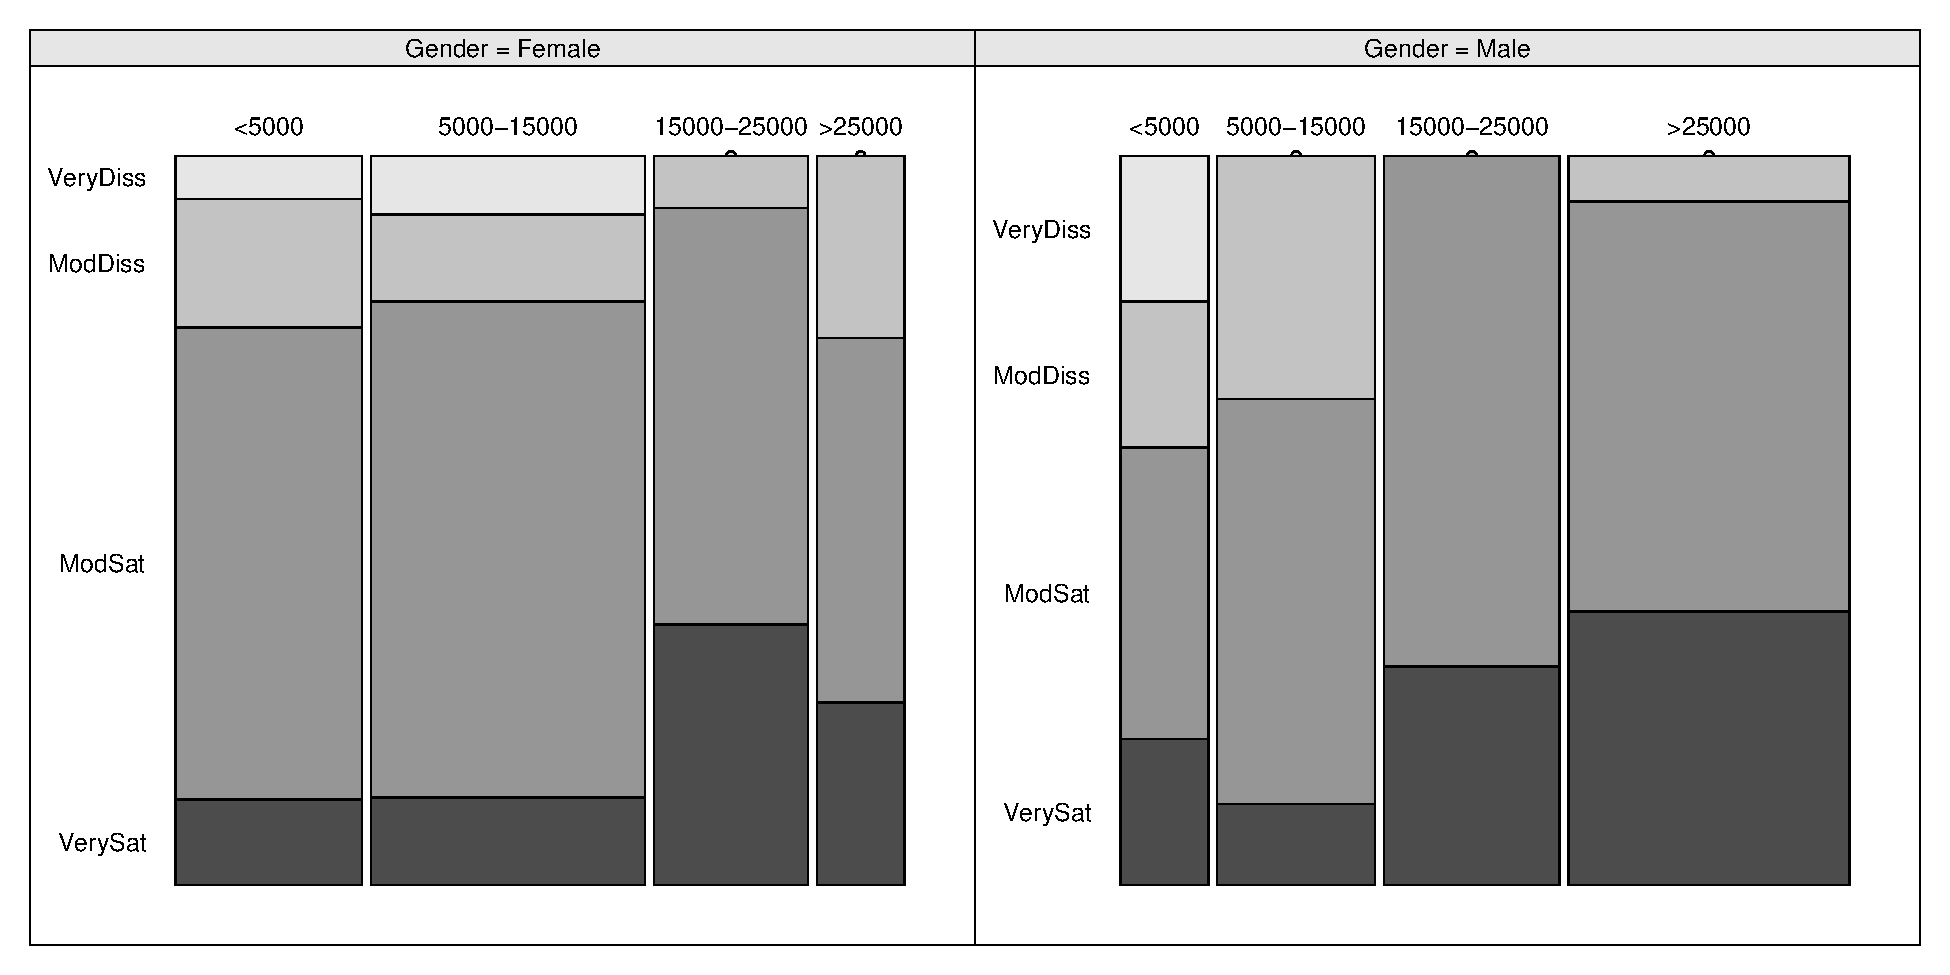
\includegraphics{coin_implementation-js-plot}
\caption{Conditional mosaic plot of job satisfaction and incoming given gender.
         \label{jsplot}}
\end{center}
\end{figure}
Here, we focus on conditional tests for independence 
of income and job satisfaction. The conditional Cochran-Mantel-Haenszel test is
based on a $c_\text{quad}$ statistic derived from the contingency table
and a $\chi^2$ approximation of the null distribution is utilized traditionally:
\begin{Schunk}
\begin{Sinput}
R> it <- independence_test(js, teststat = "quad", distribution = asymptotic())
R> it
\end{Sinput}
\begin{Soutput}
	Asymptotic General Independence Test

data:  Job.Satisfaction by
	 Income (<5000, 5000-15000, 15000-25000, >25000) 
	 stratified by Gender 
chi-squared = 10.2001, df = 9, p-value = 0.3345
\end{Soutput}
\end{Schunk}
with linear statistic
\begin{Schunk}
\begin{Sinput}
R> statistic(it, "linear")
\end{Sinput}
\begin{Soutput}
            VeryDiss ModDiss ModSat VerySat
<5000              2       4     13       3
5000-15000         2       6     22       4
15000-25000        0       1     15       8
>25000             0       3     13       8
\end{Soutput}
\end{Schunk}
This is exactly the two-way classification
\begin{Schunk}
\begin{Sinput}
R> margin.table(js, 1:2)
\end{Sinput}
\begin{Soutput}
             Job.Satisfaction
Income        VeryDiss ModDiss ModSat VerySat
  <5000              2       4     13       3
  5000-15000         2       6     22       4
  15000-25000        0       1     15       8
  >25000             0       3     13       8
\end{Soutput}
\end{Schunk}
i.e., the three-dimensional table aggregated over the block factor \code{Gender}.
This contingency table in standardized form reads
\begin{Schunk}
\begin{Sinput}
R> statistic(it, "standardized")
\end{Sinput}
\begin{Soutput}
              VeryDiss     ModDiss     ModSat    VerySat
<5000        1.3112789  0.69201053 -0.2478705 -0.9293458
5000-15000   0.6481783  0.83462550  0.5175755 -1.6257547
15000-25000 -1.0958361 -1.50130926  0.2361231  1.4614123
>25000      -1.0377629 -0.08983052 -0.5946119  1.2031648
\end{Soutput}
\end{Schunk}
Instead of using a $\chi^2$ statistic collapsing the whole table via a quadratic form, one might
want to use the maximum of the absolute values of the standardized cells as test statistic.
This maximum-type test is set up  easily:
\begin{Schunk}
\begin{Sinput}
R> independence_test(js, teststat = "max")
\end{Sinput}
\begin{Soutput}
	Asymptotic General Independence Test

data:  Job.Satisfaction by
	 Income (<5000, 5000-15000, 15000-25000, >25000) 
	 stratified by Gender 
maxT = 1.6258, p-value = 0.7214
\end{Soutput}
\end{Schunk}
with its conditional asymptotical null distribution being 
available immediately (due to the joint multivariate normal distribution
for the contingency table $\T$). Single-step adjusted $p$~values for each
cell of the contingency table corresponding to this maximum test
can be computed via
\begin{Schunk}
\begin{Sinput}
R> pvalue(independence_test(js, teststat = "max"), 
+        method = "single-step")
\end{Sinput}
\begin{Soutput}
             VeryDiss   ModDiss    ModSat   VerySat
<5000       0.9009726 0.9987769 0.9999998 0.9888039
5000-15000  0.9992718 0.9948674 0.9998852 0.7214172
15000-25000 0.9660244 0.8034652 0.9999999 0.8268942
>25000      0.9761806 1.0000000 0.9996381 0.9394831
\end{Soutput}
\end{Schunk}
Taking the ordinal scale level of both
variables into account, a linear by linear association test \citep{agresti2002}
is easily performed
\begin{Schunk}
\begin{Sinput}
R> it <- independence_test(js, 
+     scores = list(Job.Satisfaction = c(1, 3, 4, 5),
+                   Income = c(3, 10, 20, 35)),
+     distribution = approximate(B = 10000))
R> pvalue(it)
\end{Sinput}
\begin{Soutput}
[1] 0.0107
99 percent confidence interval:
 0.008233232 0.013643997 
\end{Soutput}
\end{Schunk}
For more practical examples, including applications with numeric variables, 
we refer to \cite{Hothorn:2006:AmStat}.

\section{Quality assurance}

The test procedures implemented in package \pkg{coin} are continuously
checked against results obtained by the corresponding implementations in
package \pkg{stats} (where available). In addition, the test statistics
and exact, approximate and asymptotic $p$~values for data examples
given in the \pkg{StatXact}~6 user manual \citep{StatXact6} are compared
with the results reported there. Step-down multiple adjusted $p$~values
have been checked against results reported by \Rcmd{mt.maxT} from
package \pkg{multtest} \citep{PKG:multtest}. For details on the test
procedures we refer to the \proglang{R} transcript files in directory
\code{coin/tests} of the \pkg{coin} package sources.

\section{Computational details}

The class structure, internal functionality, user interface and examples are
based on \pkg{coin} version 0.6-6, available
under the terms of the General Public License from \url{http://CRAN.R-project.org/}. 
\proglang{R} version 2.5.1 was used for 
the computations, see \url{http://www.R-project.org/}.

\section*{Acknowledgments}
 
We would like to thank Helmut Strasser for discussions on the theoretical framework.
Henric Nilsson provided clarification and examples for the Maxwell-Stuart test and helped
identifying bugs. The work of T.~Hothorn was supported by Deutsche Forschungsgemeinschaft (DFG) 
under grant HO 3242/1-3.

\bibliography{coin}

\end{document}
